\pagebreak
\section{Modelando contextos arm\'onicos}
\label{sec:harmonic_contexts}
\subsection{Contextos}
Una car'acteristica de la m'usica compartida con el lenguaje es que un mismo s'imbolo es interpretado de distinta forma seg'un el contexto
en donde este sea percibido. En el caso del lenguaje, se refiere por s'imbolo a una palabra. Esta diferencia interpretativa es conocida 
como polisemia, y refiere a la cualidad de una palabra de tener m'as de un significado. Por ejemplo, la palabra \emph{sierra}, refiere
tanto a un instrumento que permite cortar madera, como a una parte de la cordillera. De esta forma, en la oraci'on 
``Lindo viaje por la sierra'' atribuye un significado a la palabra sierra, mientras que ``Compr'e una sierra nueva, puesto que la vieja 
estaba gastada'' atribuye el otro. 

Este mismo fen'omeno ocurre con la m'usica, lo que cambia es la noci'on de \emph{contexto} y de \emph{interpretaci'on}. En este caso
la interpretaci'on estar'a relacionada con el \emph{grado de estabilidad}\footnote{El cocepto de estabilidad en este contexto est'a relacionado
con el concepto de estabilidad f'isica: Un objeto es estable si tiende a quedarse en el estado en el que est'a, sin embargo, cuando un objeto
es inestable tiende a cambiar de estado. Notas inestables generan tensi'on en direcci'on a notas estables} que genera una cierta nota, 
y el contexto estar'a dado por una pieza musical; una nota por si sola no es ni estable ni inestable, lo es en un cierto \emph{contexto}. 
A modo de ejemplo, la nota Si en la tonalidad de Si mayor es la nota m'as estable, sin embargo, esta misma nota en la tonalidad de Do mayor es llamada
\emph{sensible} por el grado de tensi'on que genera hacia Do.
Si bien es cierto que a una nota se le atribuye un grado de estabilidad en el contexto de una pieza, esta definici'on es por dem'as vaga. 
A continuaci'on se refinar'a este concepto.  

\cite{Krumhansl90} refiere a estas relaciones de estabilidad como jer'arquicas, en el sentido de que existen elementos normativos que son tomados 
como punto de referencia. Este fen'omeno no es exclusivo de la m'usica; los colores son frecuentemente descriptos respecto a ciertos colores 
focales como rojo, verde, azul, y amarillo. Los n'umeros son comparados con otros que tienen un status cognitivo especial: 9 es casi 10, 95 es casi 100. 
Si bien estas analog'ias permiten ejemplificar a qu'e se refiere por elemento normativo, existe una diferencia con la m'usica que es importante notar. 
Una nota no posee por s'i misma ninguna caracter'istica que la haga m'as suceptible a ser tomada como punto de referencia, sin embargo, ciertos
colores y n'umeros lo son. La estabilidad relativa de una nota entonces 
depender'a de factores como el contexto m'etrico en donde esta aparezca o su posici'on en el contorno de la l'inea mel'odica, entre otros. 
Se refiere entonces a estas relaciones entre notas como \texttt{la jerarqu'ia tonal}. Basada en estos principios, Krumhansl, propone m'etodos 
emp'iricos para cuantificar esta jerarqu'ia.

%Karol Krumhansl refiere en \cita a la m'usica occidental como tonal-arm'onica, haciendo referencia a dos propiedades importantes que rigen
%su coherencia. Por tonal, se refiere a el hecho de que las piezas musicales occidentales est'an organizadas al rededor de una cierta 
%nota denominada \emph{t'onica}, a su vez, por harm'onica se refiere al marco para establecer las relaciones entre las alturas respecto a la t'onica. Krumhansl contin'ua
%identificando tres elementos dentro de la musica tonal-arm'onica: alturas, acordes y tonalidades.

%Por altura se refiere a una de las posible 12 categor'ias disponibles en la m'usica tonal, por acorde, a cualquier grupo de 3 o m'as 
%notas que suenen en simult'aneo\footnote{esa es la definici'on que esta en la pagina 9\ldots no habla de superposici'on de 3ras}, y por 
%tonalidad a la t'onica y su escala, que es un patr'on de intervalos definidos en relaci'on a la t'onica. 

Por su parte, \cite{Lerdahl2001} en su libro A \texttt{Tonal Pitch Space} contin'ua en cierto sentido con el trabajo de Krumhansl, y define un espacio en donde pretende 
modelar, entre otras cosas, el grado de estabilidad de una nota en un cierto contexto, definiendo contexto a partir de dos cosas: una tonalidad y un acorde. 
Aunque su teor'ia es mucho m'as general y abarcativa, en este trabajo s'olo se tomar'an esos conceptos.

En lo que sigue, se presenta con mayor detalle parte de los estudios de Krumhansl y Lerdahl, para luego dar un marco bayesiano sobre el cual montar las jerarqu'ias tonales.

\subsection{Pitch profiles}
\label{sec:pitch_profile}
A continuaci'on se describir'a el m'etodo propuesto por Krumhansl para cuantificar el grado de estabilidad de una nota dentro de la jerarqu'ia tonal. 
El m'etodo es llamado \emph{probe tone method} y se basa en el siguiente hecho: Krumhansl observ'o en sus experimentos que cuando se presentaba a un sujeto una escala 
incompleta, esta genera una fuerte expectativa sobre el tono faltante. Por ejemplo, si sonaran las notas Do, Re, Mi, Fa, Sol, La, Si en ese orden, se generar'ia una fuerte 
expectativa de escuchar Do, y no s'olo esto, sino que este fen'omeno es independiente de la octava en la que se produzca el Do para completar.
Krumhansl denomina a esta 'ultima nota \emph{probe tone}, y su experimento se basa en exponer al oyente a todas las posibles continuaciones, y que este de un puntaje
seg'un cuan buena considera la continuaci'on escuchada. La hip'otesis es que el grado de ``buena continuaci'on'' que le era atribuido al \emph{probe tone} es funci'on
de la relaci'on que tiene este 'ultimo con la t'onica de la escala.
Una vez finalizado el experimento, se promedian las calificaciones dadas por los sujetos para construir el pitch profile.

%\red{XXX releer}
 En la figura \ref{fig:pitch_profile} se exhibe un ejemplo de pitch profile para la escalas mayor y menor: 
el eje X representa todas las alturas dentro de una escala, el eje Y es el promedio de las respuestas de los sujetos. De esta forma, se puede observar que en la escala mayor, los grados arm'onicos
1, 3 y 5 (Do, Mi y Sol - o C, E y G en la figura - en la escala de Do mayor) son los m'as estables, luego le sigue los tonos correspondientes al resto de la escala mayor, y por 'ultimo el resto de los 
tonos.


\begin{imagen}
    \file{images/pitch_profiles.png}
    \labelname{fig:pitch_profile}
    \desc{El pitch profile para m'usicos. Figura tomada de \cite{Krumhansl90}.}
    \width{10cm}
\end{imagen}


En su trabajo, Krumhansl propone distintas caracter'isticas de las notas, y las analiza mediante t'ecnicas de regresi'on, llegando a la conclusi'on que la
caracter'istica m'as importante es la duraci'on relativa de una nota respecto al resto: La nota cuya proporci\'on es mayor en la obra musical ser'a la t'onica. 
A partir de este estudio, es posible entonces inferir un pitch profile. Dado que a los efectos de generar una melod'ia no es de inter'es saber el nombre de la 
tonalidad, se propone utilizar el pitch profile como distribuci'on de probabilidades para la elecci'on de las notas.

\subsection{El espacio diat\'onico}
Hist'oricamente se han hecho una gran cantidad de intentos por encuadrar dentro de un modelo grafico/espacial las relaciones de estabilidad entre elementos de la m'usica
tonal.  \cite{Lerdahl2001} propone un espacio cuyos elementos son alturas, acordes y tonalidades. En 'el, define una noci'on de distancia que pretende 
reflejar el parentesco entre estos t'erminos de estabilidad. As'i establece tanto la estabilidad de una nota dentro de un contexto, 
como tambi'en la distancia entre dos acordes dentro de una tonalidad, o entre dos tonalidades. 
Nuevamente, dentro del alcance de esta tesis no es de inter'es medir esas distancias, sin embargo, se considera que el comportamiento que tiene el modelo de Lerdahl es deseable en un modelo estad'istico
que vaya a cuantificar la estabilidad de una nota. Se considera que se podr'ian aplicar estas nociones de distancia para poder construir melod'ias en m'usica de 
tipo modal.

El autor trabaja con la noci'on de contexto como interacci'on entre la tonalidad que rige en el tema  y el
acorde que gobierna la estabilidad en ese momento. El primero lo denomina como \emph{espacio b'asico}. 
El espacio b'asico refleja las relaciones de estabilidad que le son aplicadas a las notas en relaci'on a una tonalidad. 

En la figura \ref{fig:basic_space} se exhibe una representaci'on gr'afica del espacio tonal b'asico para la tonalidad de Do mayor. En el eje vertical, se encuentra
representado el nivel de estabilidad: Una nota que esta en el nivel \texttt{a} ser'a m'as estable que una nota que se encuentre solamente 
en un nivel inferior. Como 
podr'a verse, todas las notas se encuentran en el nivel \texttt{e}, de menor estabilidad, y a medida que se sube de nivel, s'olo un subconjunto de notas son las 
que persisten, es decir, notas de niveles superiores siempre tienen su lugar en los niveles inferiores.

\begin{figure}
\begin{center}
\begin{tabular}{r c c c c c c c c c c c c c} 
a) & Do &      &    &      &    &    &      &     &       &    &      &    & Do\\
b) & Do &      &    &      &    &    &      & Sol &       &    &      &    & Do\\
c) & Do &      &    &      & Mi &    &      & Sol &       &    &      &    & Do\\
d) & Do &      & Re &      & Mi & Fa &      & Sol &       & La &      & Si & Do\\
e) & Do & Do\# & Re & Re\# & Mi & Fa & Fa\# & Sol & Sol\# & La & La\# & Si & Do\\
\newline
\end{tabular}
\caption{ Espacio b\'asico para la tonalidad de Do mayor}
\label{fig:basic_space}
\end{center}
\end{figure}

%\begin{imagen}
%    \file{images/basic_space.png}
%    \labelname{fig:basic_space}
%    \desc{Espacio b\'asico para la tonalidad de Do mayor}
%    \width{10cm}
%\end{imagen}

De esta forma, dada una tonalidad y una nota, para saber el grado de estabilidad de esa nota basta con mirar el nivel m'as alto en el que aparece.
Luego el autor define una regla para afectar a este espacio por el contexto dado por un acorde. Cuando se refiere a afectar este contexto por un acorde, pensar
en un guitarrista cantando: A medida que van transcurriendo los acordes de la canci'on, el guitarrista va cambiando las notas que canta, inclusive podr'ia
suceder que notas que suenan muy bien ante la presencia de un cierto acorde, suenan totalmente disonantes ante la presencia de otro. 
Esta regla para afectar el espacio b'asico lo que hace es desplazar las notas m'as estables del espacio original, en nuestro ejemplo Do, Sol y Mi, de forma tal
que las nuevas notas m'as estables sean las del acorde, dejando el resto de las notas con la estabilidad que ten'ian por el espacio b'asico. 

A modo de ejemplo se exhibe el espacio desplazado para el acorde de Re menor (Re, Fa, La) en la figura \ref{fig:dm_space}

\begin{figure}[!h]
\begin{center}
\begin{tabular}{r c c c c c c c c c c c c c} 
a) &    &      & Re &      &    &    &     &      &       & La &      &    &  \\
b) &    &      & Re &      &    & Fa &     &      &       & La &      &    &  \\
c) &    &      & Re &      &    & Fa &     &      &       & La &      &    &  \\
d) & Do &      & Re &      & Mi & Fa &     &  Sol &       & La &      & Si & Do\\
e) & Do & Do\# & Re & Re\# & Mi & Fa & Fa\# & Sol & Sol\# & La & La\# & Si & Do\\
\end{tabular}
\newline
\caption{ Espacio desplazado para Re menor}
\label{fig:dm_space}
\end{center}
\end{figure}

\subsection{El modelo}
\label{sec:harmonic_context_model}
El objetivo de este modelo es cuantificar el grado de estabilidad de una nota dentro de un contexto, definiendo por contexto una tonalidad y un acorde. 
Es deseable que este modelo exhiba un comportamiento similar a lo que Lerdahl describe en su teor'ia. 

Como se mencion'o en la secci'on anterior, no es de inter'es saber el nombre de la tonalidad de la pieza musical, es por esto que como estimaci'on de la 
tonalidad se utilizar'a el pitch profile de la partitura estimado a partir de la proporci'on de tiempo que una nota suena en la pieza. Luego, bas'andose en 
la teor'ia de Lerdahl, ante la presencia de un acorde este contexto se ve afectado haciendo que las notas del acorde se conviertan en las m'as probables.  

Esto se puede analizar construyendo una distribuci'on a priori basado en el pitch profile, y actualizando esa distribuci'on a priori con la observaci'on del acorde. 
Formalmente, sea $\theta$ un vector de 12 dimensiones, donde $\theta_i$ corresponde a la probabilidad de tocar la nota $i$. Sean adem'as las notas $n_1, \cdots, n_k$ las notas 
tocadas por el acorde. Entonces estamos interesados en conocer la distribuci'on a posteriori de vector $\theta$. Utilizando la ley de bayes

$$P(\theta|n_1, \cdots, n_k) = \frac{P(n_1,\cdots, n_k | \theta) P(\theta)}{\int_{\theta}P(n_1, \cdots, n_k | \theta) P(\theta)}$$

Dado que existen 12 notas posibles, se puede considerar la elecci'on de una nota como una variable multinomial, entonces 
si se considera a $\theta \sim Dirichlet(\alpha p_1, \cdots, \alpha p_{12})$ siendo $p$ el vector del pitch profile y $\alpha$ un factor de peso sobre la creencia previa.

$$\theta | n_1, \cdots, n_k \sim Dirichlet(\alpha p_1 + \sum_{i=1}^k \delta_{n_i,1}, \cdots, \alpha p_{12} + \sum_{i=1}^k \delta_{n_i,12})$$

En la figura \ref{fig:prior_profile} exhibe el pitch profile de un fragmento del coral de Bach en Sol mayor, ``Uns ist ein Kindlein heut'', 
y luego en la figura \ref{fig:pitch_posteriors}
la distribuci'on a posteriori dado que son'o el acorde de La menor, que consta de las notas La, Do y Mi para distintos valores de $\alpha$. 
Se puede ver como si $\alpha$ toma valores grandes, el hecho
de que se haya observado el acorde pr'acticamente no influye en la distribuci'on a posteriori, puesto que la creencia previa tiene mucha fuerza, sin embargo a medida que se baja el valor se pasa por una 
distribuci'on de alguna forma uniforme entre las notas del acorde de Sol mayor y de La menor, y luego las notas de La menor pasan a ser las m'as estables.

\begin{imagen}
    \file{images/posteriors/prior-profile.png}
    \labelname{fig:prior_profile}
    \desc{Pitch profile de una pieza en Sol mayor}
    \width{10cm}
\end{imagen}

\begin{figure}[htp]
    \begin{center}
        \begin{tabular}{cc}
        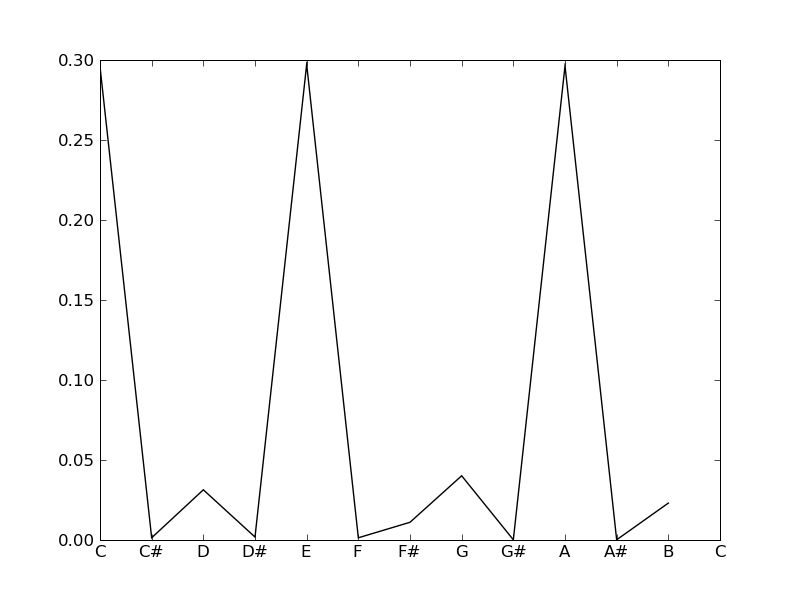
\includegraphics[width=7.5cm]{images/posteriors/posterior-profile-0_5.png} &
        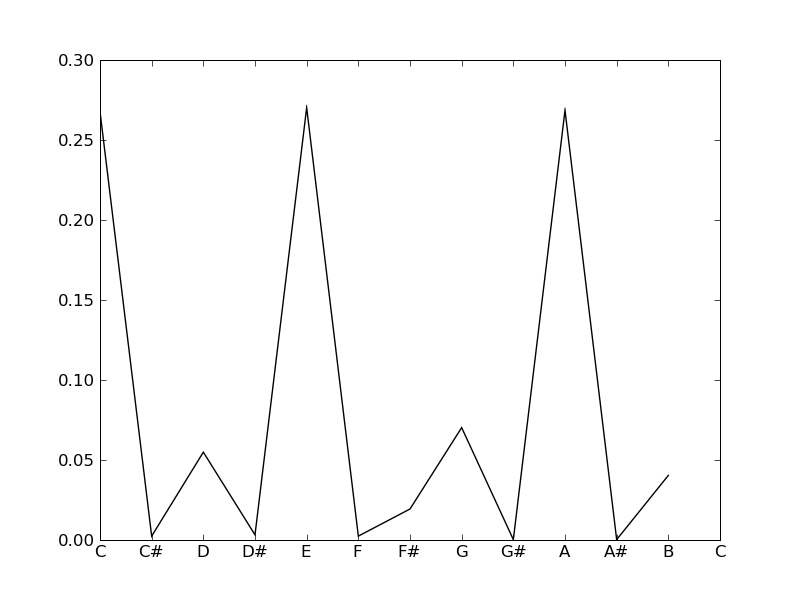
\includegraphics[width=7.5cm]{images/posteriors/posterior-profile-1.png} \\
        $\alpha=0.5$ & $\alpha=1$ \\
    %%	\vspace{1cm} & \\
        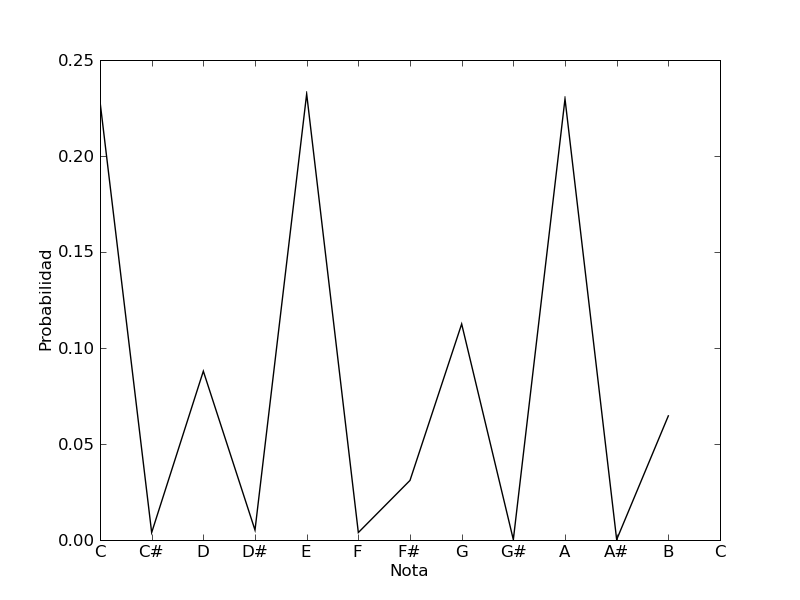
\includegraphics[width=7.5cm]{images/posteriors/posterior-profile-2.png} &
        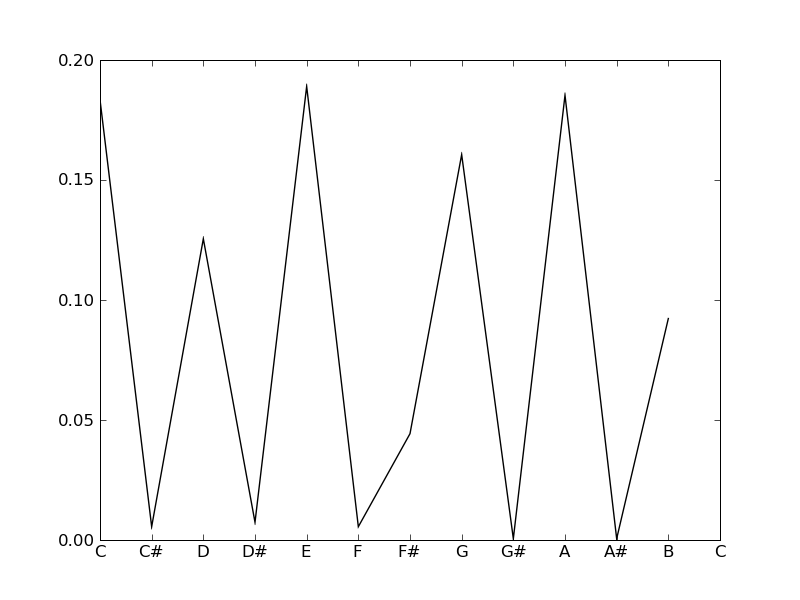
\includegraphics[width=7.5cm]{images/posteriors/posterior-profile-4.png} \\
        $\alpha=2$ & $\alpha=4$ \\
    %%	\vspace{1cm} & \\
        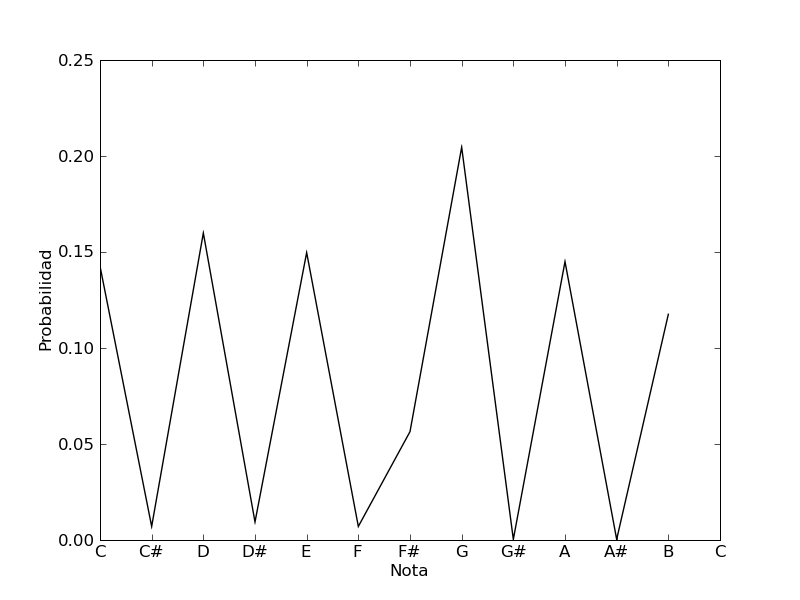
\includegraphics[width=7.5cm]{images/posteriors/posterior-profile-8.png} &
        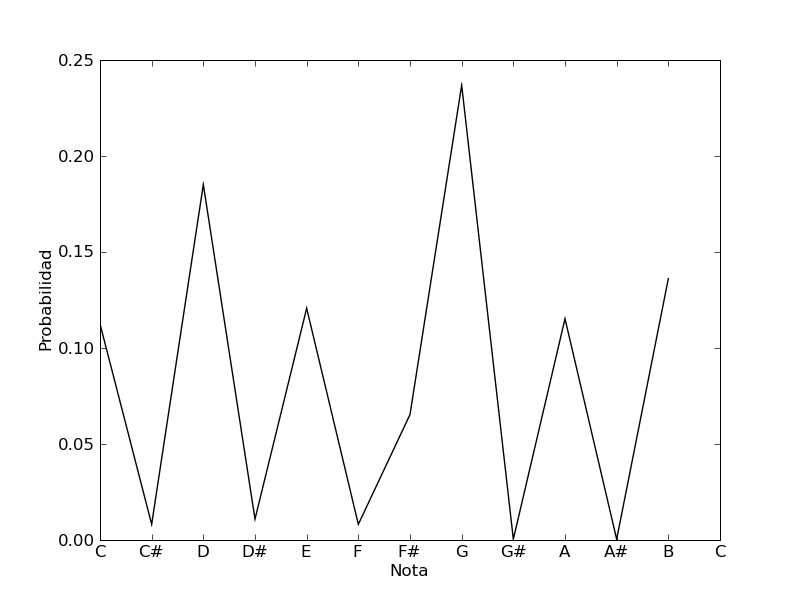
\includegraphics[width=7.5cm]{images/posteriors/posterior-profile-16.png} \\
        $\alpha=8$ & $\alpha=16$ \\
    %%	\vspace{1cm} & \\

        \end{tabular}
        \caption{Distribuciones a posteriori de un contexto arm\'onico para distintos valores de $\alpha$. Se puede ver cuando $\alpha=0.5$ el acorde de La menor 
        domina en el pitch profile, mientras que cuando $\alpha=16$ la distribuci'on predominante responde mayormente a la distribuci'on original con una leve modificaci'on
        en las notas que corresponden al acorde de La menor.}
        \label{fig:pitch_posteriors}
    \end{center}      
\end{figure}

El modelo planteado en esta secci'on hace ciertas asunciones impl'icitas de las que se desea dar detalle. 
Si bien Krumhansl propone al pitch profile Krumhansl como mecanismo para caracterizar la tonalidad en la que se encuentra una pieza, 
podr'ia no ser ser suficiente para generar una melod'ia que sea entendida de la misma forma. 
Como primer variac'ion, en lugar de que la probabilidad de una nota sea la proporci'on de tiempo que esta son'o en el tiempo, 
se podr'ia construir una familia de distribuci'ones indexadas por su duraci'on. 'Esta ser'ia otra forma de reflejar el hecho de que notas que 
suenan m'as tiempo tienden a ser estables.

Obs'ervese que el peso que se le da a cada nota del acorde es igual. En ese caso podr'ia plantearse el modelo en otros t'erminos para permitir un factor de peso, o
alg'un tipo de condici'on que distinga entre cada nota. 

Otra caracter'istica que no es tenida en cuenta en este modelo es el acento m'etrico que recibe una cierta nota. Es sabido que en posiciones m'etricamente m'as fuertes
existen restricci'ones sobre la estabilidad de las notas que se pueden tocar all'i. Nuevamente, una soluci'on podr'ia ser tener una familia de distribuci'ones indexadas
por el acentro m'etrico. Esto mismo ocurre tambi'en con las notas que reciben un acento estructural, sin embargo en la secci'on \ref{sec:phrases} se dar'a una posible
soluci'on a este problema. 

\section{Sobre la detecci\'on de acordes}
Para implementar el modelo propuesto en esta secci'on fue necesario desarrollar una heur'istica para la detecci'on de acordes puesto que la entrada no los trae anotados. 
Esta heur'istica es relativamente simple y se basa en las notas
que suenan en simult'aneo, eliminando las notas que son equivalentes bajo la equivalencia entre octavas. Luego refina el resultado descartando candidatos a acordes que suenan en simult'aneo y no se organizan en saltos de 3 o 4 semitonos, por ejemplo Do, Re, Mi. 

Hay un caso a tener en cuenta, y es que en general, cuando se tocan acordes
con s'eptima, como Do, Mi, Sol, Si$\flat$ se suele obviar la quinta, en este caso Sol. De esta forma, en la partitura se observar'an que las notas Do, Mi, Si$\flat$ suenan
en simult'aneo, y ser'ian falsamente descartadas.  Es por esto que la heur'istica de detecci'on de acordes trata de completar 
con una nota en caso de haber fallado al organizar las notas de a saltos de 3 o 4 semitonos para asi poder inferir el acorde de tr'iada correspondiente (en 
el caso de Do, Mi, Si$\flat$ completar a Do, Mi, Sol, Si$\flat$ e inferir Do, Mi, Sol). 

Queda como trabajo a futuro trabajar con arpegios, es decir, sucesiones de notas que conforman un acorde pero que no son tocadas en simultaneo. 
Se cree que podr'ia atacarse este problema mediante un algoritmo de \emph{changepoint detection}\footnote{El lector interesado en \emph{changepoint detection} refi'erase 
a \cite{adams-mackay-2007}}, para detectar los cambios en el foco tonal. Los algoritmos de changepoint 
detection permiten detectar los puntos de cambio de una sucesi'on de medici'ones en donde la distribuci'on de probabilidades subyacente cambia abruptamente.
A nivel ilustrativo, un ejemplo concreto es el efecto que tiene a la percepci'on de un robot prender la luz de una habitaci'on: Todos las entradas visuales 
sufren un cambio abrupto en su distribuci'on subyacente, de esta forma la estimaci'on que se ten'ia hasta el momento no sirve. En el caso de un cambio
en el foco tonal, la distribuci'on que sufrir'ia un cambio ser'ia la propuesta en esta secci'on, de esta forma, cambios en la distribuci'on a posteriori, indicar'ian
cambios en el foco tonal.

\section{Ejemplos}
Al igual que con el modelo de la m'etrica, se generaron ejemplos de melod'ias siguiendo los modelos definidos en esta secci'on. Para 
cada pieza de entrada se compuso una melod'ia siguiendo un 'unico pitch profile, correspondiente a la tonalidad inferida, y otra
afectando el pitch profile con los acordes detectados. Los ejemplos se encuentran disponibles en 
\url{http://elsonidoq.tzulberti.webfactional.com/examples/?section_name=harmonic_context}.
